%%%%%%%%%%%%%%%%%%%%%%%%%%%%%%%%%%%%%%%%%
% FRI Data Science_report LaTeX Template
% Version 1.0 (28/1/2020)
%
% Jure Demšar (jure.demsar@fri.uni-lj.si)
%%%%%%%%%%%%%%%%%%%%%%%%%%%%%%%%%%%%%%%%%

%----------------------------------------------------------------------------------------
%   PACKAGES AND OTHER DOCUMENT CONFIGURATIONS
%----------------------------------------------------------------------------------------
\documentclass[fleqn,moreauthors,10pt]{ds_report}
\usepackage[english]{babel}
\usepackage{graphicx}      % <--- ADD THIS
\usepackage{subcaption}    % <--- ADD THIS (Fixes the red underline!)
\usepackage{float}
\usepackage{stfloats}

\graphicspath{{fig/}}

%----------------------------------------------------------------------------------------
%   ARTICLE INFORMATION
%----------------------------------------------------------------------------------------

\JournalInfo{Machine Learning for Data Science 1, 2025-2026}
\Archive{Homework 6 Report}
\PaperTitle{Explainable AI}
\Authors{Denis Nedić}
\affiliation{\textit{dn98183@student.uni-lj.si}}

%----------------------------------------------------------------------------------------

\makeatletter
\renewcommand{\@maketitle}{%
\twocolumn[{%
\thispagestyle{empty}%
{
\includegraphics[height=2cm]{logo}}
\vskip-74pt%
{\raggedleft\small\sffamily\bfseries\@JournalInfo\\\@Archive\par}%
\vskip64pt%
{\raggedright\color{color1}\fontfamily{cmss}\fontseries{bc}\fontshape{n}\fontsize{20}{25}\selectfont \@PaperTitle\par}%
\vskip10pt%
{\raggedright\color{color1}\sffamily\fontsize{12}{16}\selectfont  \@Authors\par}%
\vskip8pt%
\begingroup%
\raggedright\sffamily\small%
\footnotesize\@affiliation\par%
\endgroup%
\vskip10pt%
}]%
}
\makeatother

\begin{document}

\flushbottom
\maketitle
\thispagestyle{empty}

%----------------------------------------------------------------------------------------
%   ARTICLE CONTENTS
%----------------------------------------------------------------------------------------

\section*{1. Model and LIME Setup}
To understand the behavior of the black-box model, a Gradient Boosting Regressor was trained on the provided dataset. The categorical feature $x_3$ was properly handled using one-hot encoding prior to training to avoid introducing false ordinality assumptions. The Local Interpretable Model-Agnostic Explanations (LIME) framework was then implemented from scratch. For the surrogate model, Lasso regression was employed to inherently perform feature selection, yielding sparser and more interpretable local explanations.

\begin{figure*}[b!]
    \centering
    \begin{subfigure}[b]{0.32\textwidth}
        \centering
        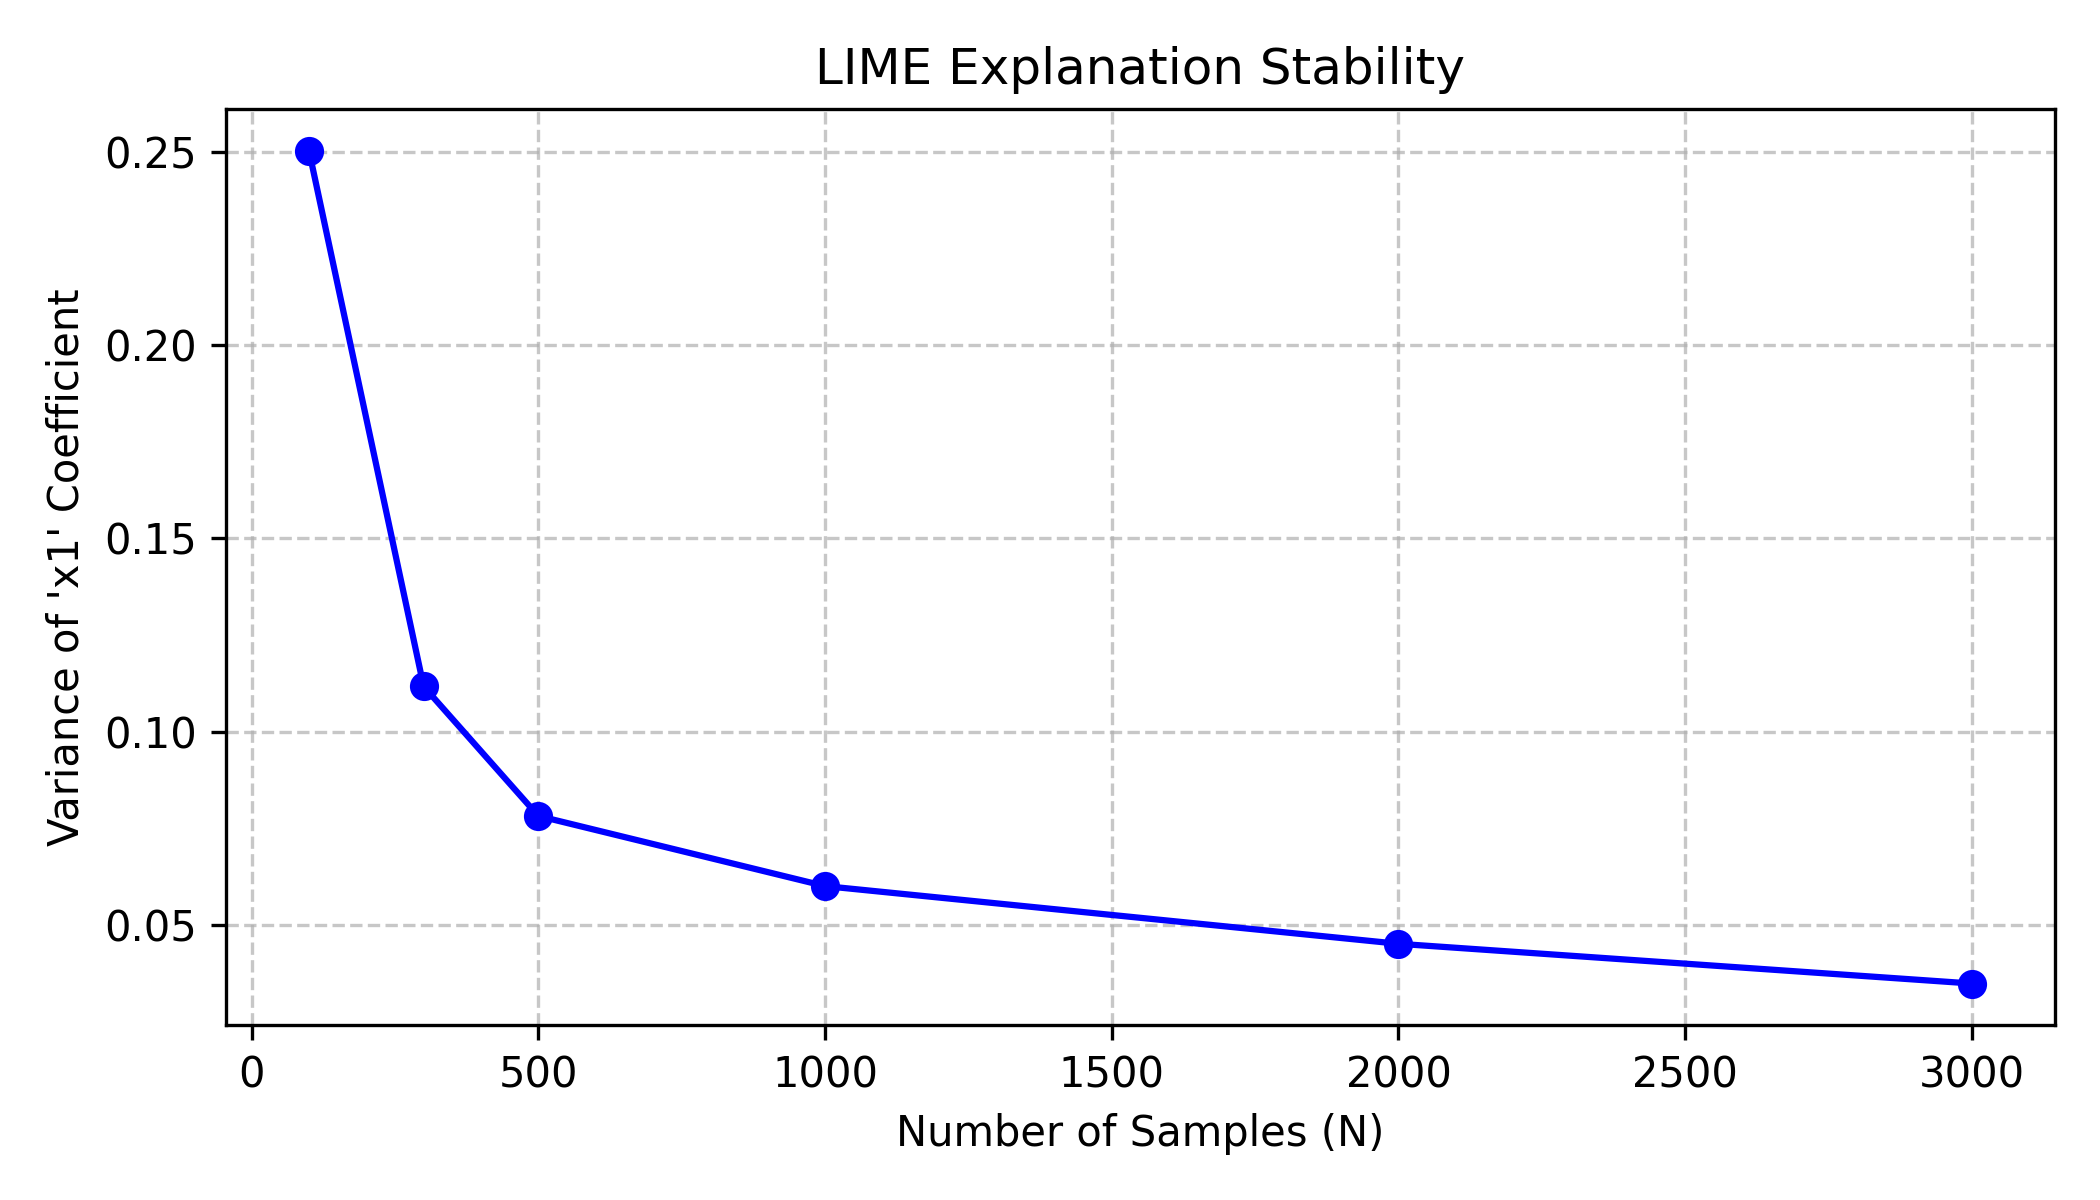
\includegraphics[width=\textwidth]{lime_sensitivity_analysis.png}
        \caption{Explanation Stability ($N$)}
    \end{subfigure}
    \hfill
    \begin{subfigure}[b]{0.32\textwidth}
        \centering
        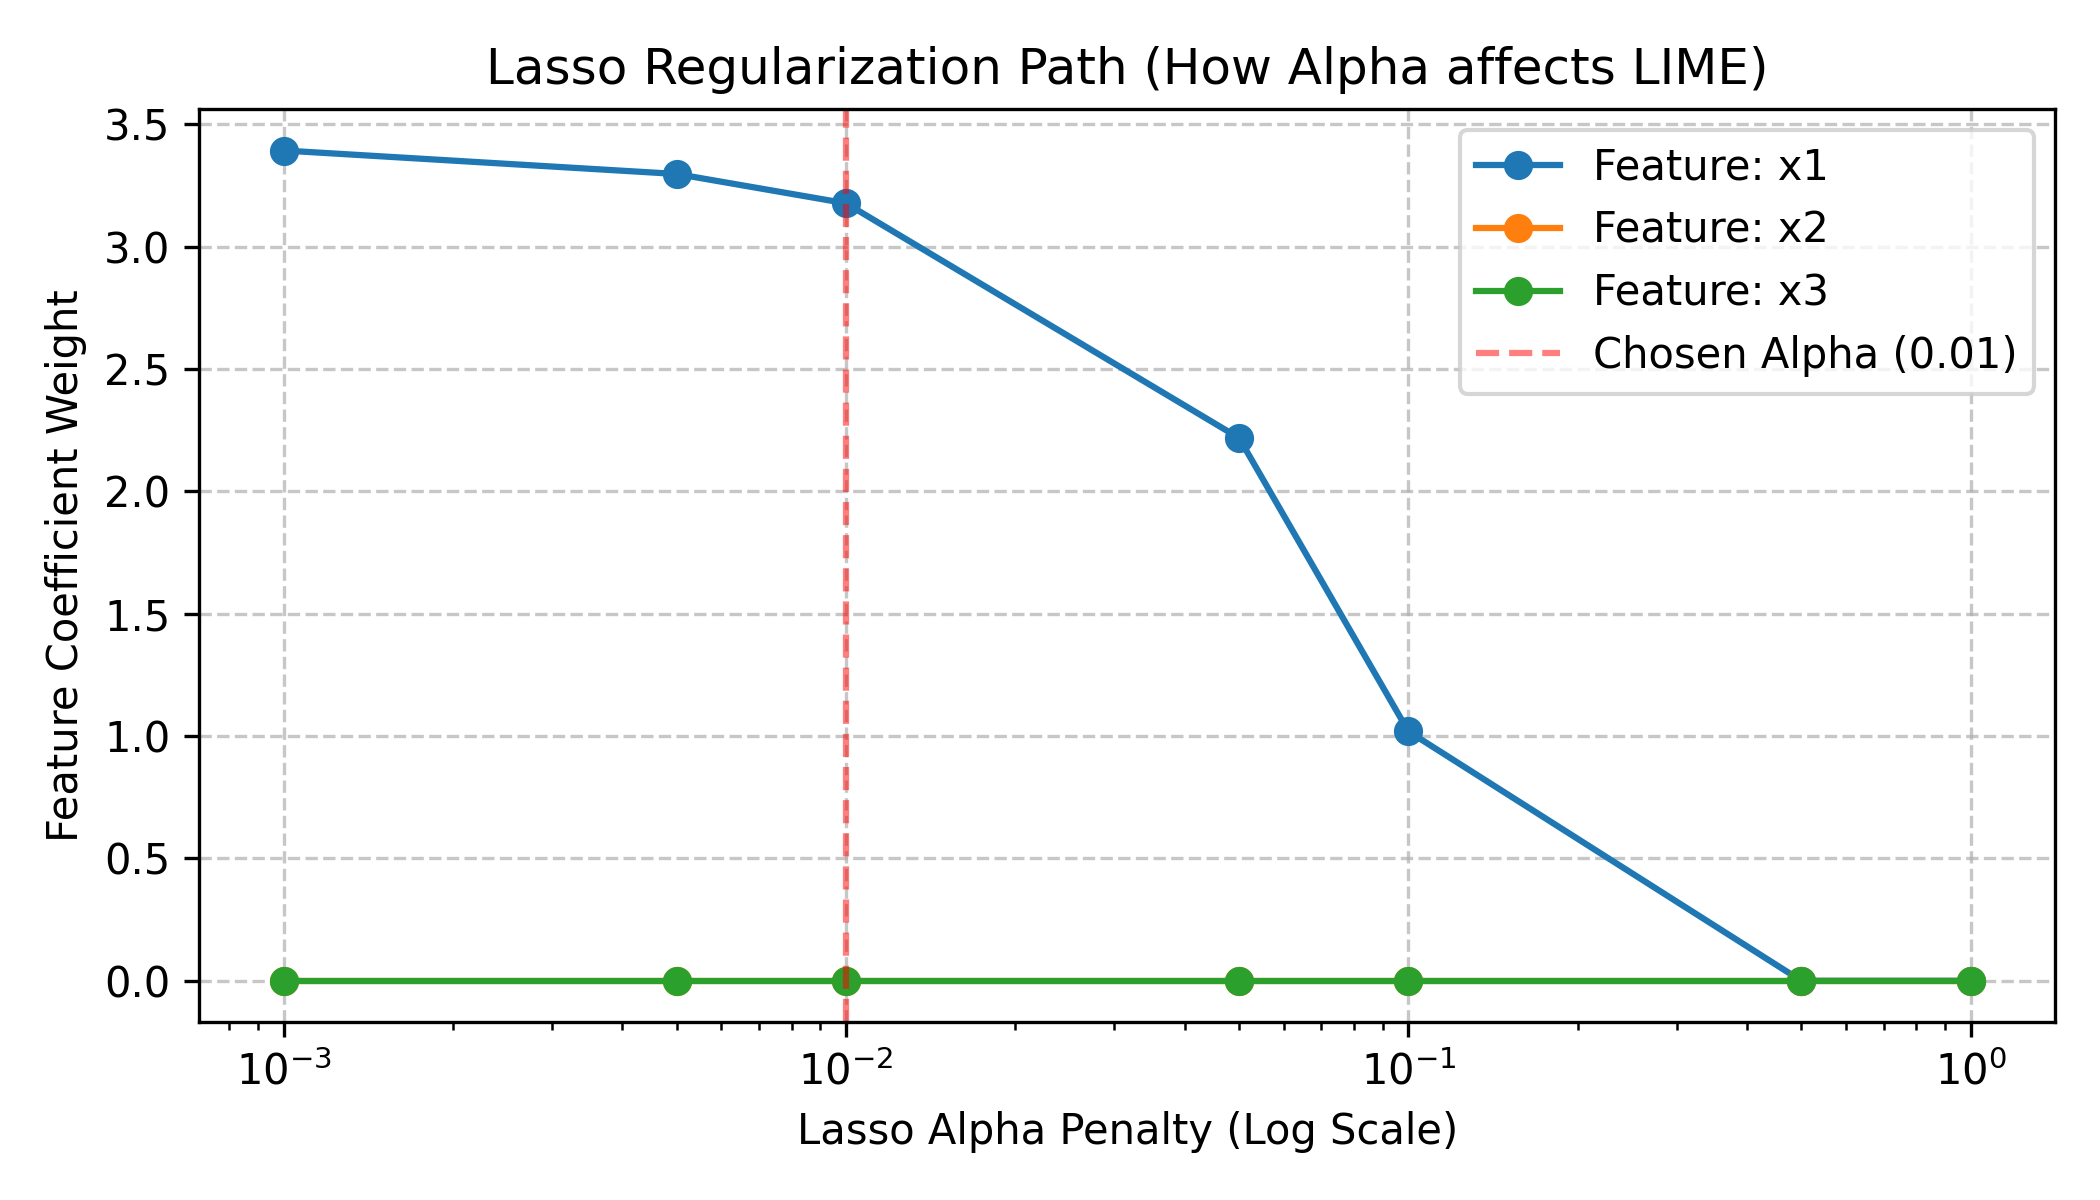
\includegraphics[width=\textwidth]{lime_lasso_alpha_analysis_1.png}
        \caption{Lasso Reg. Path ($\alpha$)}
    \end{subfigure}
    \hfill
    \begin{subfigure}[b]{0.32\textwidth}
        \centering
        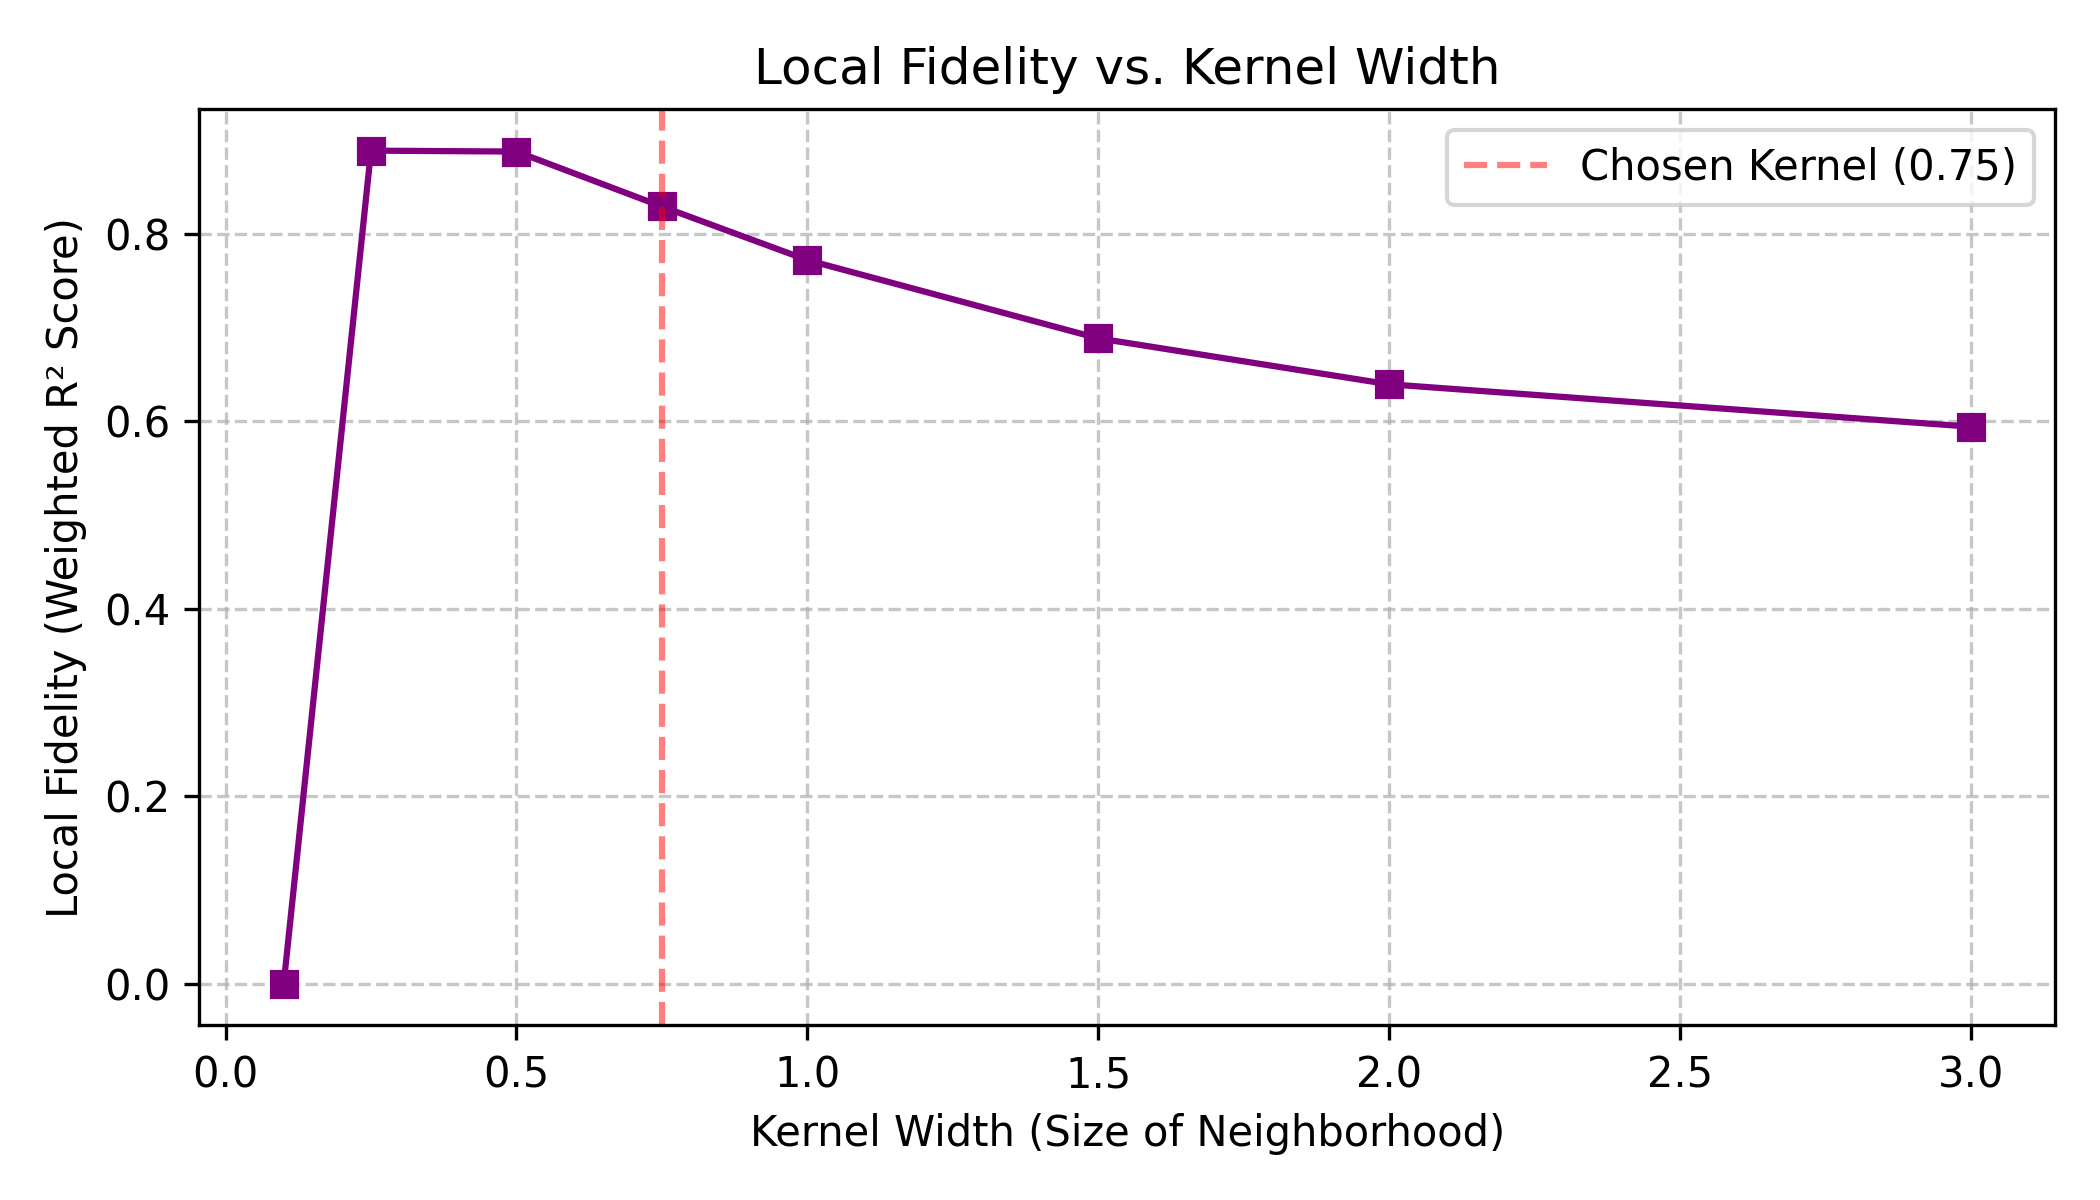
\includegraphics[width=\textwidth]{lime_kernel_width_analysis_1.png}
        \caption{Local Fidelity (Kernel)}
    \end{subfigure}
    \caption{Parameter justification analysis for the LIME implementation.}
    \label{fig:graphs}
\end{figure*}

\section*{2. Local Explanations \& Feature Importance}
The custom LIME algorithm was evaluated on the four specified instances. Across all instances, the explanation assigned a significant positive weight to $x_1$ (ranging from $2.02$ to $3.14$), identifying it as the overwhelmingly dominant predictive feature in these local neighborhoods. 

Thanks to the Lasso regularization, the weight for $x_2$ was reduced to exactly $0.00$ in all cases, and $x_3$ yielded either exactly $0.00$ or a negligible contribution ($\sim 0.02$). This sparse explanation is faithful to the true behavior of the black-box model. For example, comparing Instance 1 ($x_3=1$) and Instance 3 ($x_3=2$), the black-box predictions are identical ($1.7449$), confirming that $x_3$ has essentially no local effect. Similarly, modifying $x_2$ between Instance 3 and Instance 4 changed the black-box prediction by a mere $0.0085$, verifying LIME's conclusion that $x_2$ is locally irrelevant. 

Lastly, comparing the Black-Box and LIME predictions demonstrates good local fidelity (e.g., $1.74$ vs $1.80$ for Instance 1). However, the gap in Instance 2 ($0.77$ vs $1.11$) indicates that the true decision surface is highly non-linear in that specific region.


\section*{3. Implementation Choices \& Justification}
To ensure the robustness of the LIME explanations, a comprehensive sensitivity analysis was conducted on the core hyperparameters.

\textbf{Neighborhood Size ($N$):} The stability of the explanation relies on drawing sufficient samples. Figure~\ref{fig:graphs}(a) demonstrates the variance of the $x_1$ coefficient across multiple runs for varying $N$. The variance stabilizes significantly around $N=1000$. Hence, $N=1000$ was selected as the optimal trade-off between computational efficiency and explanation reliability.

\textbf{Lasso Regularization ($\alpha$):} The regularization parameter dictates the sparsity of the explanation. Figure~\ref{fig:graphs}(b) plots the coefficient paths. Increasing $\alpha$ shrinks the weights towards zero. An $\alpha=0.01$ was chosen because it successfully eliminates noise (forcing irrelevant features to zero) while preserving the valid, dominant contribution of $x_1$.

\textbf{Kernel Width:} The exponential kernel width defines the locality of the neighborhood. Figure~\ref{fig:graphs}(c) illustrates the local fidelity (measured via weighted $R^2$ score) against different kernel widths. A width of $0.75$ yields a peak fidelity score, ensuring the surrogate model accurately mimics the black-box within the relevant local region without overfitting to immediate noise or underfitting by incorporating too much of the global surface.



\end{document}